\documentclass[a4paper]{article}
\usepackage{geometry}
\usepackage{graphicx}
\usepackage{natbib}
\usepackage{amsmath}
\usepackage{amssymb}
\usepackage{amsthm}
\usepackage{paralist}
\usepackage{epstopdf}
\usepackage{tabularx}
\usepackage{longtable}
\usepackage{multirow}
\usepackage{multicol}
\usepackage[hidelinks]{hyperref}
\usepackage{fancyvrb}
\usepackage{algorithm}
\usepackage{algorithmic}
\usepackage{float}
\usepackage{paralist}
\usepackage[svgname]{xcolor}
\usepackage{enumerate}
\usepackage{array}
\usepackage{times}
\usepackage{url}
\usepackage{fancyhdr}
\usepackage{comment}
\usepackage{environ}
\usepackage{times}
\usepackage{textcomp}
\usepackage{caption}
\usepackage{multirow}


\urlstyle{rm}

\setlength\parindent{0pt} % Removes all indentation from paragraphs
\theoremstyle{definition}
\newtheorem{definition}{Definition}[]
\newtheorem{conjecture}{Conjecture}[]
\newtheorem{example}{Example}[]
\newtheorem{theorem}{Theorem}[]
\newtheorem{lemma}{Lemma}
\newtheorem{proposition}{Proposition}
\newtheorem{corollary}{Corollary}


\floatname{algorithm}{Procedure}
\renewcommand{\algorithmicrequire}{\textbf{Input:}}
\renewcommand{\algorithmicensure}{\textbf{Output:}}
\newcommand{\abs}[1]{\lvert#1\rvert}
\newcommand{\norm}[1]{\lVert#1\rVert}
\newcommand{\RR}{\mathbb{R}}
\newcommand{\CC}{\mathbb{C}}
\newcommand{\Nat}{\mathbb{N}}
\newcommand{\br}[1]{\{#1\}}
\DeclareMathOperator*{\argmin}{arg\,min}
\DeclareMathOperator*{\argmax}{arg\,max}
\renewcommand{\qedsymbol}{$\blacksquare$}

\definecolor{dkgreen}{rgb}{0,0.6,0}
\definecolor{gray}{rgb}{0.5,0.5,0.5}
\definecolor{mauve}{rgb}{0.58,0,0.82}

\newcommand{\Var}{\mathrm{Var}}
\newcommand{\Cov}{\mathrm{Cov}}

\newcommand{\vc}[1]{\boldsymbol{#1}}
\newcommand{\xv}{\vc{x}}
\newcommand{\Sigmav}{\vc{\Sigma}}
\newcommand{\alphav}{\vc{\alpha}}
\newcommand{\muv}{\vc{\mu}}

\newcommand{\red}[1]{\textcolor{red}{#1}}

\def\x{\mathbf x}
\def\y{\mathbf y}
\def\w{\mathbf w}
\def\v{\mathbf v}
\def\E{\mathbb E}
\def\V{\mathbb V}

% TO SHOW SOLUTIONS, include following (else comment out):
\newenvironment{soln}{
    \leavevmode\color{blue}\ignorespaces
}{}


\hypersetup{
%    colorlinks,
    linkcolor={red!50!black},
    citecolor={blue!50!black},
    urlcolor={blue!80!black}
}

\geometry{
  top=1in,            % <-- you want to adjust this
  inner=1in,
  outer=1in,
  bottom=1in,
  headheight=3em,       % <-- and this
  headsep=2em,          % <-- and this
  footskip=3em,
}


\pagestyle{fancyplain}
\lhead{\fancyplain{}{Homework 3}}
\rhead{\fancyplain{}{CS 760 Machine Learning}}
\cfoot{\thepage}

\title{\textsc{Homework 3}} % Title

%%% NOTE:  Replace 'NAME HERE' etc., and delete any "\red{}" wrappers (so it won't show up as red)

\author{
\red{$>>$Nevindu M. Batagoda$<<$} \\
\red{$>>$9081677594$<<$}\\
} 

\date{}

\begin{document}

\maketitle 


\textbf{Instructions:} 
Use this latex file as a template to develop your homework. Submit your homework on time as a single pdf file to Canvas. Late submissions may not be accepted. Please wrap your code and upload to a public GitHub repo, then attach the link below the instructions so that we can access it. You can choose any programming language (i.e. python, R, or MATLAB). Please check Piazza for updates about the homework.

\section{Questions (50 pts)}
\begin{enumerate}
\item (9 pts) Explain whether each scenario is a classification or regression problem. And, provide the number of data points ($n$) and the number of features ($p$).

\begin{enumerate}
	\item (3 pts) We collect a set of data on the top 500 firms in the US. For each firm we record profit, number of employees, industry and the CEO salary. We are interested in predicting CEO salary with given factors.
	
	\begin{soln} 
		This is a regression problem, as the CEO salary is a continuous numeric variable. There are $n=500$ data points and $p=3$ features, where the features are profit, number of employees, and industry. 
	\end{soln}
	
	\item (3 pts) We are considering launching a new product and wish to know whether it will be a success or a failure. We collect data on 20 similar products that were previously launched. For each product we have recorded whether it was a success or failure, price charged for the product, marketing budget, competition price, and ten other variables.
	
	\begin{soln}
		This is a classification problem, as the outcome is a binary variable (success or failure). There are $n=20$ data points and $p=13$ features, where the features are price charged for the product, marketing budget, competition price, and ten other variables.
	\end{soln}
	
	\item (3 pts) We are interesting in predicting the \% change in the US dollar in relation to the weekly changes in the world stock markets. Hence we collect weekly data for all of 2012. For each week we record the \% change in the dollar, the \% change in the US market, the \% change in the British market, and the \% change in the German market.
	
	\begin{soln}
		This is a regression problem, as the \% change in the US dollar is a continuous numeric variable. There are $n=52$ data points and $p=3$ features, where the features are the \% change in the US market, the \% change in the British market, and the \% change in the German market.
	\end{soln}
	
\end{enumerate}

\item (6 pts) The table below provides a training data set containing six observations, three predictors, and one qualitative response variable.

\begin{center}
	\begin{tabular}{ c  c  c  c}
		\hline
		$X_{1}$ & $X_{2}$ & $X_{3}$ & $Y$ \\ \hline
		0 & 3 & 0 & Red \\
		2 & 0 & 0 & Red \\
		0 & 1 & 3 & Red \\
		0 & 1 & 2 & Green \\
		-1 & 0 & 1 & Green \\
		1 & 1 & 1 & Red  \\
		\hline
	\end{tabular}
\end{center}

Suppose we wish to use this data set to make a prediction for $Y$ when $X_{1} = X_{2} = X_{3} = 0$ using K-nearest neighbors.

\begin{enumerate}
	\item (2 pts) Compute the Euclidean distance between each observation and the test point, $X_{1} = X_{2} = X_{3}=0$.
 
	\begin{soln} 
		Let $x = (0, 0, 0)$ be the test point. Then the Euclidean distance between each observation and the test point is as follows.
		\begin{align*}
			\text{Observation 1} & : ||x - x_1||_2^2 = \sqrt{(0-0)^2 + (3-0)^2 + (0-0)^2} = 3 \\
			\text{Observation 2} & : ||x - x_2||_2^2 =\sqrt{(2-0)^2 + (0-0)^2 + (0-0)^2} = 2 \\
			\text{Observation 3} & : ||x - x_3||_2^2 =\sqrt{(0-0)^2 + (1-0)^2 + (3-0)^2} = \sqrt{10} = 3.16\\
			\text{Observation 4} & : ||x - x_4||_2^2 =\sqrt{(0-0)^2 + (1-0)^2 + (2-0)^2} = \sqrt{5} = 2.24\\
			\text{Observation 5} & : ||x - x_5||_2^2 =\sqrt{(-1-0)^2 + (0-0)^2 + (1-0)^2} = \sqrt{2} = 1.41\\
			\text{Observation 6} & : ||x - x_6||_2^2 =\sqrt{(1-0)^2 + (1-0)^2 + (1-0)^2} = \sqrt{3} = 1.73\\
		\end{align*}
	\end{soln}
 
	\item (2 pts) What is our prediction with $K=1$? Why?
	
	\begin{soln}
		Our prediction with $K=1$ is Green, because the nearest neighbor to the test point is Observation 5, with a distance $1.41$, which is Green.
		
	\end{soln}
	
	\item (2 pts) What is our prediction with $K=3$? Why?
	
	\begin{soln} 
		Our prediction with $K=3$ is Red, because the three nearest neighbors to the test point are Observation 5, Observation 6, and Observation 2, with distances $1.41$, $1.73$, and $2$, respectively. Among these three neighbors, two of them are Red and one of them is Green. Therefore, the prediction is Red.
	\end{soln}

\end{enumerate}

\item (12 pts) When the number of features $p$ is large, there tends to be a deterioration in the performance of KNN and other local approaches that perform prediction using only observations that are near the test ob- servation for which a prediction must be made. This phenomenon is known as the curse of dimensionality, and it ties into the fact that non-parametric approaches often perform poorly when $p$ is large.

\begin{enumerate}
	\item (2pts) Suppose that we have a set of observations, each with measurements on $p=1$ feature, $X$. We assume that $X$ is uniformly (evenly) distributed on [0, 1]. Associated with each observation is a response value. Suppose that we wish to predict a test observation’s response using only observations that are within 10\% of the range of $X$ closest to that test observation. For instance, in order to predict the response for a test observation with $X=0.6$, we will use observations in the range [0.55, 0.65]. On average, what fraction of the available observations will we use to make the prediction?
	
	\begin{soln} 
		Since $X$ is uniformly distributed on $[0,1]$, any subinterval of length $k$ contains a fraction $k$ of the observations. Therefore, the fraction of the available observations we will use to make the prediction is $0.1$.		 
	\end{soln}
	
	
	\item (2pts) Now suppose that we have a set of observations, each with measurements on $p =2$ features, $X1$ and $X2$. We assume that predict a test observation’s response using only observations that $(X1,X2)$ are uniformly distributed on [0, 1] × [0, 1]. We wish to are within 10\% of the range of $X1$ and within 10\% of the range of $X2$ closest to that test observation. For instance, in order to predict the response for a test observation with $X1 =0.6$ and $X2 =0.35$, we will use observations in the range [0.55, 0.65] for $X1$ and in the range [0.3, 0.4] for $X2$. On average, what fraction of the available observations will we use to make the prediction?
	
	\begin{soln} 
		Since $X1$ and $X2$ are uniformly distributed on $[0,1]$, any subinterval of length $k$ contains a fraction $k$ of the observations. Therefore, The fraction of the available observations we will use to make the prediction is the area of the square with side length $0.1$, which is $0.1^2 = 0.01$.
		
	\end{soln}
	
	\item (2pts) Now suppose that we have a set of observations on $p = 100$ features. Again the observations are uniformly distributed on each feature, and again each feature ranges in value from 0 to 1. We wish to predict a test observation’s response using observations within the 10\% of each feature’s range that is closest to that test observation. What fraction of the available observations will we use to make the prediction?
	
	\begin{soln} 
		Since each feature ranges in value from 0 to 1, the fraction of the available observations we will use to make the prediction is the volume of the hypercube with side length $0.1$, which is $0.1^{100}$.
	
	\end{soln}
	
	\item (3pts) Using your answers to parts (a)–(c), argue that a drawback of KNN when p is large is that there are very few training observations “near” any given test observation.
	
	\begin{soln} 
		As the dimensionality $p$ increases, the fraction of the available observations we will use to make the prediction decreases exponentially. Therefore, there are very few training observations “near” any given test observation. 	Because of this we are basing the prediction on very few observations, which will lead to a high variance in the prediction. Also, the bias of the prediction will also be high. Furthermore, the computational cost of KNN will be high as well as we have to compute the distance between the test observation and all the training observations only to look at a very small fraction of the training observations.
	
	\end{soln}
	
	\item (3pts) Now suppose that we wish to make a prediction for a test observation by creating a $p$-dimensional hypercube centered around the test observation that contains, on average, 10\% of the training observations. For $p =$1, 2, and 100, what is the length of each side of the hypercube? Comment what happens to the length of the sides as $\lim_{{p \to \infty}}$.
	
	\begin{soln}  
		Case $p=1$: The length of each side of the hypercube is $0.1$. As it is just a one dimensional line. \\

		Case $p=2$: To get $10\%$ of the training observations we need a square with an area of $0.1$. Therefore, the length of each side of the hypercube is $\sqrt{0.1} = 0.316$. \\

		Case $p=100$: To get $10\%$ of the training observations we need a hypercube with a volume of $0.1$. Therefore, the length of each side of the hypercube is $\sqrt[100]{0.1} = 0.977$. \\

		Case as $p \to \infty$:We have the limit, $\lim_{p \to \infty}$ $\sqrt[p]{0.1} = 1$. Therefore, as $p$ increases the length of each side of the hypercube approaches $1$. That is, for an infinite dimensional space, the closest 10\% of the training observations will be all the training observations.
	\end{soln}
	
\end{enumerate}

\item (6 pts) Supoose you trained a classifier for a spam detection system. The prediction result on the test set is summarized in the following table.
\begin{center}
	\begin{tabular}{l l | l l}
		&          & \multicolumn{2}{l}{Predicted class} \\
		&          & Spam           & not Spam           \\
		\hline
		\multirow{2}{*}{Actual class} & Spam     & 8              & 2                  \\
		& not Spam & 16             & 974               
	\end{tabular}
\end{center}

Calculate
\begin{enumerate}
	\item (2 pts) Accuracy
	\begin{soln} 
		Accuracy = $\frac{TP + TN}{TP + TN + FP + FN} = \frac{8 + 974}{8 + 974 + 16 + 2} = \frac{982}{1000} = 0.982$
	\end{soln}
	\item (2 pts) Precision
	\begin{soln} 
		Precision = $\frac{TP}{TP + FP} = \frac{8}{8 + 16} = \frac{8}{24} = 0.333$
	\end{soln}
	\item (2 pts) Recall
	\begin{soln}
		Recall = $\frac{TP}{TP + FN} = \frac{8}{8 + 2} = \frac{8}{10} = 0.8$
	\end{soln}
\end{enumerate}


\item (9pts) Again, suppose you trained a classifier for a spam filter. The prediction result on the test set is summarized in the following table. Here, "+" represents spam, and "-" means not spam.

\begin{center}
\begin{tabular}{ c  c }
\hline
Confidence positive & Correct class \\ \hline
0.95 & + \\
0.85 & + \\
0.8 & - \\
0.7 & + \\
0.55 & + \\
0.45 & - \\
0.4 & + \\
0.3 & + \\
0.2 & - \\
0.1 & - \\
\hline
\end{tabular}
\end{center}

\begin{enumerate}
	\item (6pts) Draw a ROC curve based on the above table.
	
	\begin{soln} 
		\begin{figure}[H]
			\centering
			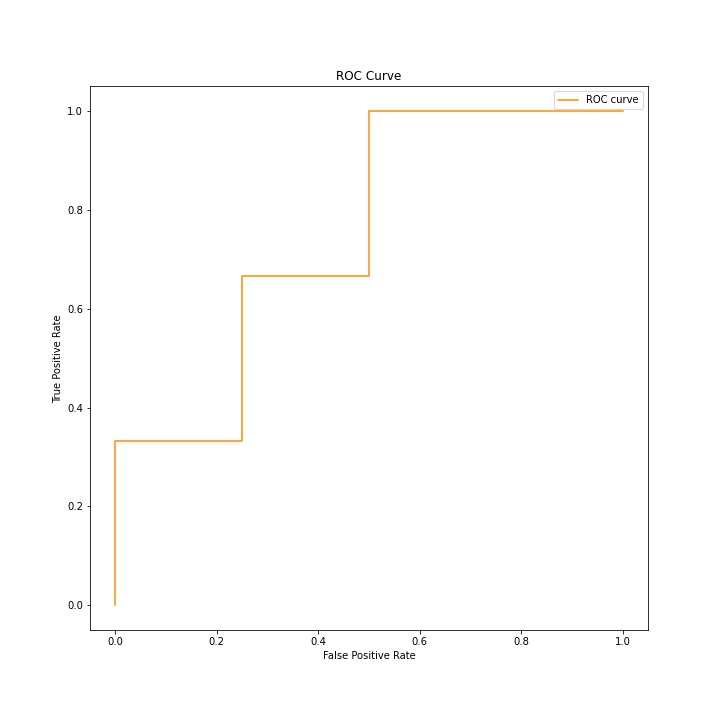
\includegraphics[width=6cm]{q1q5.jpg}
		\end{figure}
	
	\end{soln}
	
	\item (3pts) (Real-world open question) Suppose you want to choose a threshold parameter so that mails with confidence positives above the threshold can be classified as spam. Which value will you choose? Justify your answer based on the ROC curve.
	
	\begin{soln} 
		In a real-world scenario, one would like to avoid classifying a non-spam mail as spam. Therefore, it would be optimal to choose a threshold parameter such that the false positive is minimzed and the true positive rate is maximized. From the ROC curve, we can see that the therehsold value that minimize the false positive rate and maximized the true positive rate is $0.85$. This threshold gives a false positive rate of $0\%$ and a true positive rate of $33\%$. Therefore, I would choose $0.85$ as the threshold parameter. \\ 

		Note that athough there are threshold values that give a higher true positive rate, they also give a higher false positive rate. Therefore, I would choose the threshold value that gives the highest true positive rate while minimizing the false positive rate.
	\end{soln}
\end{enumerate}

\item (8 pts) In this problem, we will walk through a single step of the gradient descent algorithm for logistic regression. As a reminder,
$$\hat{y} = f(x, \theta)$$
$$f(x;\theta) = \sigma(\theta^\top x)$$
$$\text{Cross entropy loss } L(\hat{y}, y) = -[y \log  \hat{y} + (1-y)\log(1-\hat{y})]$$
$$\text{The single update step } \theta^{t+1} = \theta^{t} - \eta \nabla_{\theta} L(f(x;\theta), y) $$



\begin{enumerate}
	\item (4 pts) Compute the first gradient $\nabla_{\theta} L(f(x;\theta), y)$.
	
	\begin{soln}  
		First let's compute the derivative of the sigmoid function. $\sigma(z) = \frac{1}{1 + \exp{(-z)}}$
		\begin{align*}
			\frac{d}{dz} \sigma(z) &= \frac{d}{dz} \frac{1}{1 + \exp{(-z)}} \\
			&= \frac{d}{dz} (1 + \exp{(-z)})^{-1} \\
			&= -(1 + \exp{(-z)})^{-2} \exp{(-z)} \\
			&= \frac{\exp{(-z)}}{(1 + \exp{(-z)})^2} \\
			&= \frac{1}{(1 + \exp{(-z)})} \frac{\exp{(-z)}}{(1 + \exp{(-z)})} \\
			&= \sigma(z) (1 - \frac{1}{1+\exp{(-z)}})\\
			&= \sigma(z) (1 - \sigma(z)) \\
		\end{align*}

		Now let's compute the derivative of the cross entropy loss function. $L(\hat{y}, y) = -[y \log  \hat{y} + (1-y)\log(1-\hat{y})]$ with respect to $\theta^i$,

		\begin{align*}
			\frac{d}{d\theta^i} L(\hat{y}, y) &= \frac{d}{d\theta^i} -[y \log  \hat{y} + (1-y)\log(1-\hat{y})] \\
			&= -[y \frac{d}{d\theta^i} \log  \hat{y} + (1-y)\frac{d}{d\theta^i}\log(1-\hat{y})] \\
			&= -[y \frac{d}{d\theta^i} \log  \sigma(\theta^\top x) + (1-y)\frac{d}{d\theta^i}\log(1-\sigma(\theta^\top x))] \\
			&= -[\frac{y}{\sigma(\theta^\top x)} \frac{d}{d\theta^i} \sigma(\theta^\top x) + \frac{1-y}{1-\sigma(\theta^\top x)}\frac{d}{d\theta^i}(1-\sigma(\theta^\top x))] \\
			&= -[\frac{y}{\sigma(\theta^\top x)} \sigma(\theta^\top x) (1 - \sigma(\theta^\top x)) \frac{d}{d\theta^i} \theta^\top x + \frac{1-y}{1-\sigma(\theta^\top x)} (-\sigma(\theta^\top x) (1 - \sigma(\theta^\top x))) \frac{d}{d\theta^i} \theta^\top x] \\
			&= -[\frac{y}{\sigma(\theta^\top x)} \sigma(\theta^\top x) (1 - \sigma(\theta^\top x)) x^i + \frac{1-y}{1-\sigma(\theta^\top x)} (-\sigma(\theta^\top x) (1 - \sigma(\theta^\top x))) x^i] \\
			&= -[y(1 - \sigma(\theta^\top x)) + (1-y) (-\sigma(\theta^\top x) )]x^i \\
			&= -[y - y\sigma(\theta^\top x) - \sigma(\theta^\top x) + y\sigma(\theta^\top x)]x^i \\
			&= -[y - \sigma(\theta^\top x)]x^i \\
			&= [\sigma(\theta^\top x) - y]x^i \\
			&= [\hat{y} - y]x^i \\
		\end{align*}
	\end{soln}
	
	\item (4 pts)
 Now assume a two dimensional input. After including a bias parameter for the first dimension, we will have $\theta\in\mathbb{R}^3$.
$$ \text{Initial parameters : }  \theta^{0}=[0, 0, 0]$$
$$ \text{Learning rate }\eta=0.1$$
$$ \text{data example : } x=[1, 3, 2], y=1$$
Compute the updated parameter vector $\theta^{1}$ from the single update step.
	
	\begin{soln} 
		First, lets compute the predicted value $\hat{y} = f(x, \theta) = \sigma(\theta^\top x) = \sigma(\theta_0 + \theta_1 x_1 + \theta_2 x_2) = \sigma(\theta_0 + \theta_1 + \theta_2) = \sigma(0 + 0 + 0) = \sigma(0) = 0.5$.

		Let's compute the updated parameter vector $\theta^{1}$ from the single update step. $\theta^{t+1} = \theta^{t} - \eta \nabla_{\theta} L(f(x;\theta), y)$
		\begin{align*}
			\theta^{1} &= \theta^{0} - \eta \nabla_{\theta} L(f(x;\theta), y) \\
			&= \theta^{0} - \eta [\hat{y} - y]x \\
			&= [0, 0, 0]^T - 0.1 [\hat{y} - y]x \\
			&= [0, 0, 0]^T - 0.1 [f(x;\theta) - y]x \\
			&= [0, 0, 0]^T - 0.1 [f([1, 3, 2];[0, 0, 0]) - 1][1, 3, 2]^T \\
			&= [0, 0, 0]^T - 0.1 [0.5 - 1][1, 3, 2]^T \\
			&= [0, 0, 0]^T - 0.1 [-0.5, -1.5, -1]^T \\
			&= [0, 0, 0]^T + [0.05, 0.15, 0.1]^T \\
			&= [0.05, 0.15, 0.1]^T \\
		\end{align*}
	\end{soln}
\end{enumerate}
\end{enumerate}

\section{Programming (50 pts)}
\begin{enumerate}
	\item (10 pts) Use the whole D2z.txt as training set.  Use Euclidean distance (i.e. $A=I$).
	Visualize the predictions of 1NN on a 2D grid $[-2:0.1:2]^2$.
	That is, you should produce test points whose first feature goes over $-2, -1.9, -1.8, \ldots, 1.9, 2$, so does the second feature independent of the first feature.
	You should overlay the training set in the plot, just make sure we can tell which points are training, which are grid.
	
	The expected figure looks like this.
	\begin{figure}[H]
		\centering
		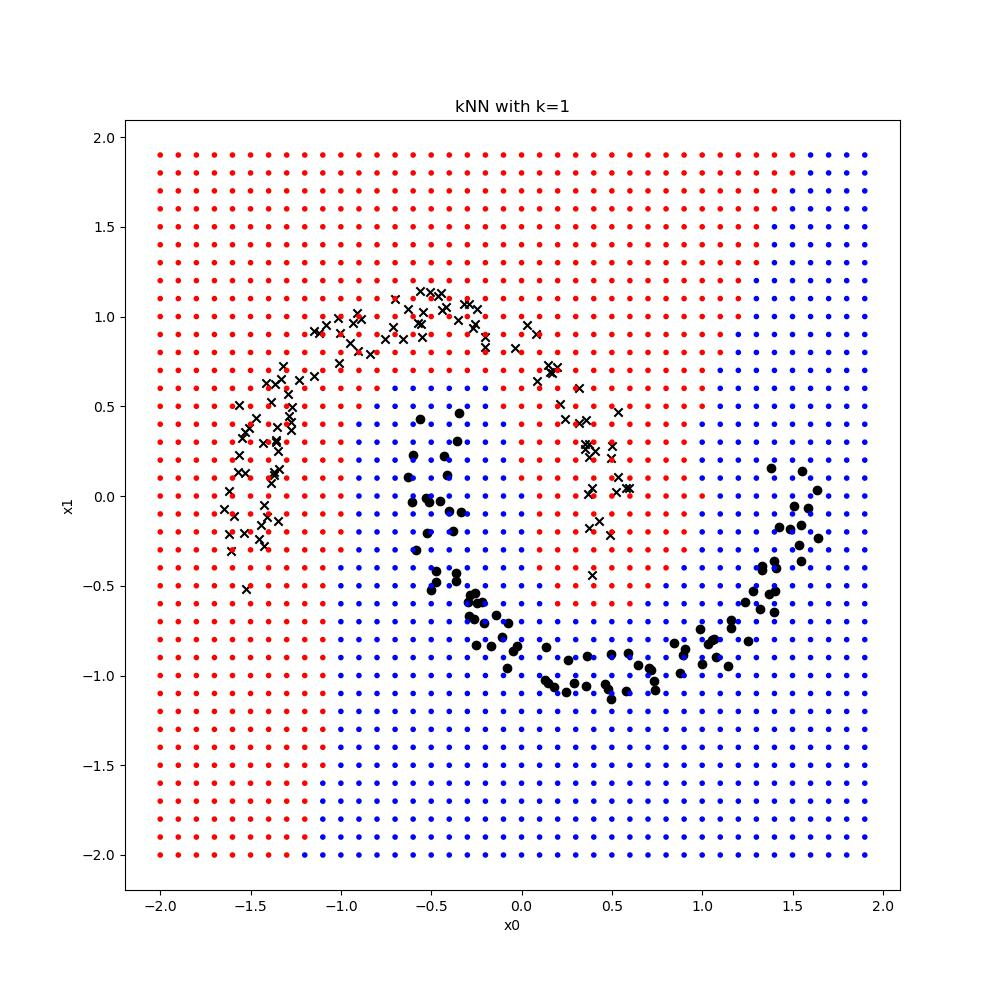
\includegraphics[width=6cm]{q2q1.jpg}
	\end{figure}
	
	\paragraph{Spam filter} Now, we will use 'emails.csv' as our dataset. The description is as follows.
	% \begin{figure}[h]
	% 	\centering
	% 	\includegraphics[width=\linewidth]{email_head.png}
	% \end{figure}
	
	\begin{itemize}
		\item Task: spam detection
		\item The number of rows: 5000
		\item The number of features: 3000 (Word frequency in each email)
		\item The label (y) column name: `Predictor'
		\item For a single training/test set split, use Email 1-4000 as the training set, Email 4001-5000 as the test set.
		\item For 5-fold cross validation, split dataset in the following way.
		\begin{itemize}
			\item Fold 1, test set: Email 1-1000, training set: the rest (Email 1001-5000)
			\item Fold 2, test set: Email 1000-2000, training set: the rest
			\item Fold 3, test set: Email 2000-3000, training set: the rest
			\item Fold 4, test set: Email 3000-4000, training set: the rest
			\item Fold 5, test set: Email 4000-5000, training set: the rest			
		\end{itemize}
	\end{itemize}
	
	\item (8 pts) Implement 1NN, Run 5-fold cross validation. Report accuracy, precision, and recall in each fold.
	
	\begin{soln} 
		\begin{table}[H]
			\centering
			\begin{tabular}{|l|l|l|l|}
			\hline
			\multicolumn{1}{|c|}{\textbf{Fold}} & \multicolumn{1}{c|}{\textbf{Accuracy}} & \multicolumn{1}{c|}{\textbf{Precision}} & \multicolumn{1}{c|}{\textbf{Recall}} \\ \hline
			Fold 1                              & 0.825                                  & 0.654                                   & 0.821                                \\ \hline
			Fold 2                              & 0.855                                  & 0.690                                   & 0.866                                \\ \hline
			Fold 3                              & 0.863                                  & 0.722                                   & 0.842                                \\ \hline
			Fold 4                              & 0.854                                  & 0.722                                   & 0.820                                \\ \hline
			Fold 5                              & 0.775                                  & 0.606                                   & 0.761                                \\ \hline
			\end{tabular}
			\end{table}
	\end{soln}
	
	\item (12 pts) Implement logistic regression (from scratch). Use gradient descent (refer to question 6 from part 1) to find the optimal parameters. You may need to tune your learning rate to find a good optimum. Run 5-fold cross validation. Report accuracy, precision, and recall in each fold.
	
	\begin{soln}
	
		\begin{table}[H]
			\centering
			\begin{tabular}{|l|l|l|l|}
			\hline
			\multicolumn{1}{|c|}{\textbf{Fold}} & \multicolumn{1}{c|}{\textbf{Accuracy}} & \multicolumn{1}{c|}{\textbf{Precision}} & \multicolumn{1}{c|}{\textbf{Recall}} \\ \hline
			Fold 1                              & 0.907                                  & 0.869                                   & 0.793                                \\ \hline
			Fold 2                              & 0.804                                  & 0.589                                   & 0.964                                \\ \hline
			Fold 3                              & 0.892                                  & 0.833                                   & 0.775                                \\ \hline
			Fold 4                              & 0.878                                  & 0.847                                   & 0.714                                \\ \hline
			Fold 5                              & 0.847                                  & 0.776                                   & 0.703                                \\ \hline
			\end{tabular}
			\end{table}
	\end{soln}
	
	\item (10 pts) Run 5-fold cross validation with kNN varying k (k=1, 3, 5, 7, 10). Plot the average accuracy versus k, and list the average accuracy of each case.


	\begin{soln}
		
	\begin{figure}[h]
		\centering
		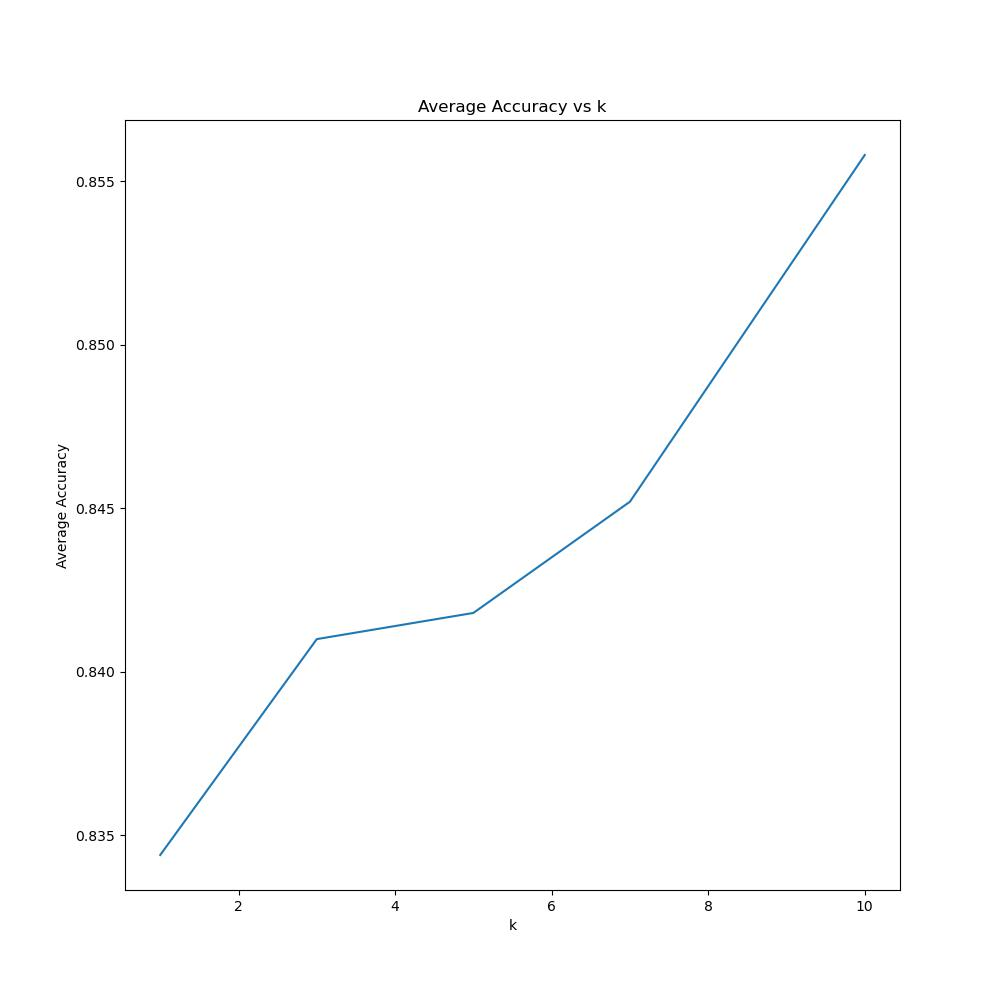
\includegraphics[width=10cm]{q2q4.jpg}
	\end{figure}
	
	
	\end{soln}
	
	\item (10 pts) Use a single training/test setting. Train kNN (k=5) and logistic regression on the training set, and draw ROC curves based on the test set.
	
	Note that the logistic regression results may differ.
	
	\begin{soln} 
		\begin{figure}[H]
			\centering
			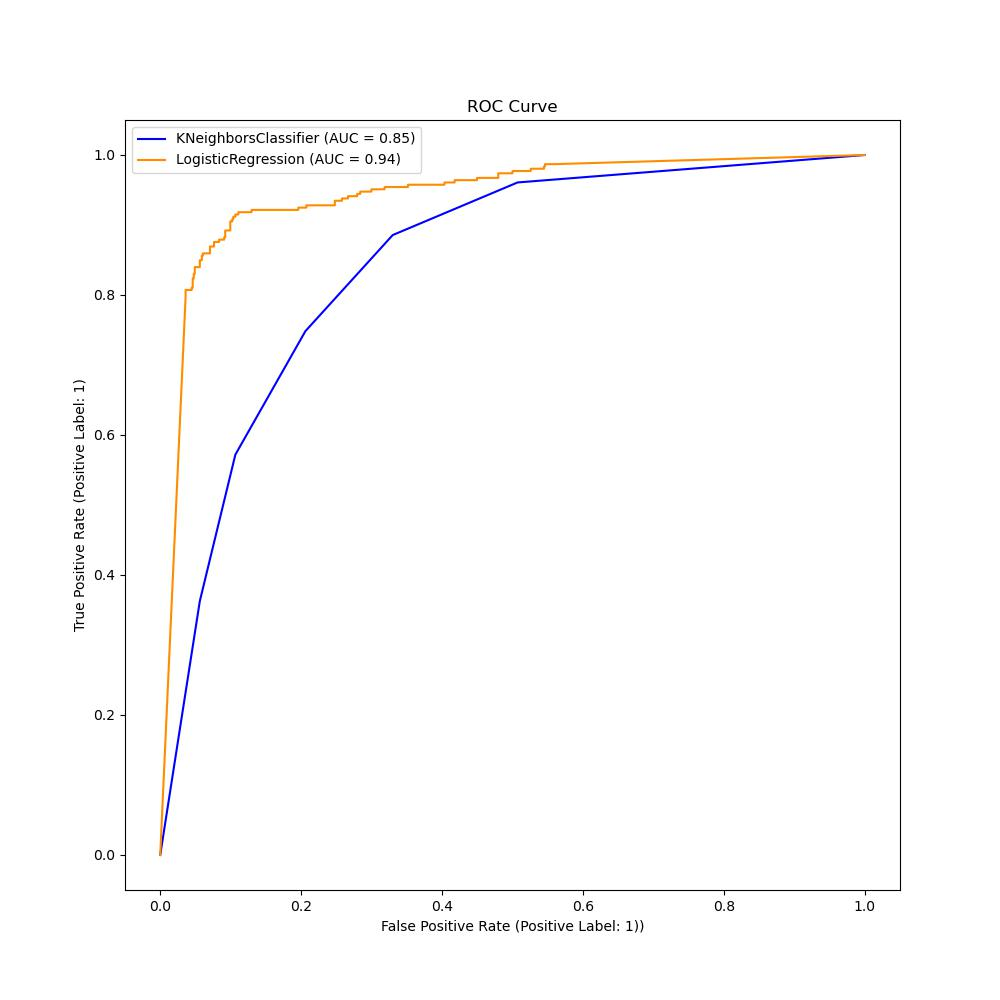
\includegraphics[width=8cm]{q2q5.jpg}
		\end{figure}
	\end{soln}
	
\end{enumerate}
\bibliographystyle{apalike}
\end{document}
